\documentclass[a4paper,11pt]{article} 
\usepackage[utf8]{inputenc} 
\usepackage{geometry} %geometry para margenes
\usepackage{circuitikz} 
\usepackage{tikz} 
\usepackage{float}
\usepackage{graphicx}
\usepackage{subcaption}
\usepackage{amssymb}
\usepackage{adjustbox}
\usepackage{fancyhdr}
\usepackage{xcolor}

\title{\textbf{Técnicas de medición}} 
\author{Deniso Xocuis}
\date{23 de marzo de 2023}
\geometry{top=2cm, bottom=2cm, left=2cm, right= 2cm}
\graphicspath{{images/}}
\parindent=0pt

\begin{document}
\maketitle
\thispagestyle{empty}
\tableofcontents %%%%%%%%%%%%%%%%%%%%%%
\noindent me costó muchisimo hacer estos apuntes, casi 10 horas investigando muchas cosas, espero sea de utilidad :D
\newpage
\setcounter{page}{1}
\pagestyle{headings}
%%%%%%%%%%%%%%%%%%%%%%Circuito en serie%%%%%%%%%%%%%%%%%%%%%%%%%
\section{Circuito en serie}
\subsection{Divisor de voltaje}
\noindent Varias resistencias en un circuito en serie en realidad es como tomar una y distribuirla.  La suma de ellas es R total, los resistores se pueden reordenar como sean y la corriente NO cambiará. 
\begin{center}

    $V_{R_n} = \frac{V*R_n}{R_T}$ \textcolor[cmyk]{1,0,1,0}{\textbf{\textit{(fórmula de divisor de voltaje)}}}
    
\end{center}
\begin{figure}[H]
    \centering
     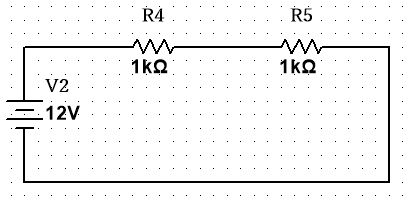
\includegraphics[width=0.4\textwidth]{images/circuito en serie.PNG}
     \caption{Circuito sencillo en serie}
     \label{fig:cs}
\end{figure}
\noindent Aquí lo que sucede es que el voltaje se divide en determinado número de resistencias de la siguiente manera:
\begin{figure}[H]
    \centering
    \begin{subfigure}{0.4\textwidth}
        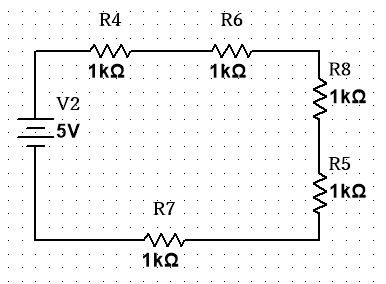
\includegraphics[width=0.9\linewidth]{images/serie.PNG}
        \caption{Circuito común en serie}
        \label{fig:cs2}
    \end{subfigure}
    \begin{subfigure}{0.4\textwidth}
        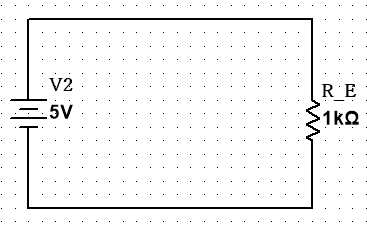
\includegraphics[width=0.9\linewidth]{images/equivalente.PNG}
        \caption{Circuito común en serie con resistencia equivalente}
        \label{fig:cs2E}
    \end{subfigure}
\end{figure}


%%%%%%%%%%%%%%%%%%%%%%Circuito en paralelo%%%%%%%%%%%%%%%%%%%%%%%%%
\section{Circuito en paralelo}
\subsection{Divisor de corriente}
\noindent La corriente se divide entre cada cable ya que tiene que regresar y dar la vuelta completa hasta el lado negativo del voltaje. En estos casos el voltaje NO cambia y la corriente va a variar  entre los cables por los diferentes valores de resistencia en cada resistor, en estos casos se puede sacar una resistencia y corriente equivalente:
\begin{center}
    
    $R_E$ = $(R_1^{-1}$ + $R_2^{-1}$....$R_n^{-1})^{-1}$ $\leftrightsquigarrow$  $R_E = \frac{R_1R_2}{R_1+R_2}$ \textcolor[cmyk]{1,0,1,0}{\textbf{\textit{(fórmulas de resistencia equivalente)}}}
    \vspace{0.2cm}\\
    $I_E$ = $\Sigma$ $\leftrightsquigarrow$ $I_E$ = I($\frac{R_n}{R_n+R_E}$) \textcolor[cmyk]{1,0,1,0}{\textbf{\textit{(fórmulas de corriente equivalente)}}}
\end{center}
\subsection{Leyes de Kirchhoff}
\noindent \begin{enumerate}
    \item Se dice que la suma algebráica de las corrientes incidentes  aun nodo coincide con la suma algebráica de las corrientes salientes del mismo (divisor de corriente). I = $I_1$ + $I_2$ ... + $I_n$ \textcolor[cmyk]{1,0,1,0}{\textbf{\textit{(fórmula de Ley de Corrientes de Kirchhoff)}}}
    \item En un circuito la suma algebráica de las caídas de voltajes en torno a cualquier lazo cerrado es igual a cero. +V-$V_{R1} - V_{R2}-...V_{Rn} = 0$ \textcolor[cmyk]{1,0,1,0}{\textbf{\textit{(fórmula de Ley de Voltaje de Kirchhoff)}}}
\end{enumerate}

\begin{figure}[H]
    \centering
     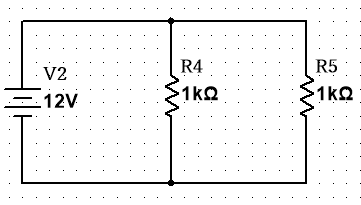
\includegraphics[width=0.4\textwidth]{images/paralelo.PNG}
     \caption{Circuito en paralelo}
     \label{fig:cp}
\end{figure}
%%%%%%%%%%%%%%%%%%%%%%Circuitos MIXTOOSS%%%%%%%%%%%%%%%%%%%%%%%%%
\section{Circuitos mixtos}
\subsection{Ejercicio de divisor de corriente y voltaje}
\noindent Sacar el divisor de voltaje del siguiente circuito:

\begin{figure}[H]
    \centering
     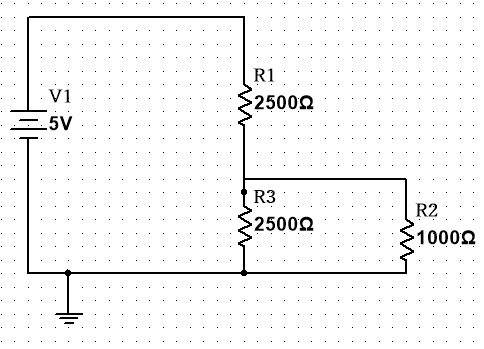
\includegraphics[width=0.5\textwidth]{images/circuito mixto1.PNG}
     \caption{Circuito mixto}
     \label{fig:cm}
\end{figure}
\noindent Lo que se ve en el circuito es que podemos sacar una resistencia equivalente en $R_3$ y $R_2$ usando la fórmula de divisor de corriente de la siguiente forma:
\vspace{0.2cm}\\
$R_E$ = (2500$^{-1}$ + 1000$^{-1}$)$^{-1}$

$R_E$ = 714.285 $\Omega$
\vspace{0.2cm}\\
\noindent De la misma forma se puede sacar la resistencia equivalente con la segunda fórmula, demostrando:
\vspace{0.2cm}\\
$R_E = \frac{R_1R_2}{R_1+R_2}$
\vspace{0.3cm}\\
$R_E = \frac{2500x1000}{2500+1000}$
\vspace{0.3cm}\\
$R_E$ = 714.285 $\Omega$
\newpage
Nos quedaría algo de la siguiente manera:

\begin{figure}[H]
    \centering
     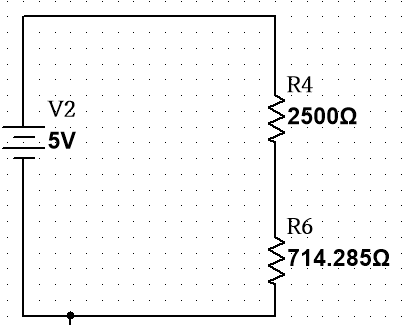
\includegraphics[width=0.3\textwidth]{images/equivalente2.PNG}
     \caption{Circuito con resistencia equivalente}
     \label{fig:E}
\end{figure}
\noindent De esta forma será mas sencilla calcular el divisor de voltaje con la siguiente fórmula:
\vspace{0.2cm}\\
$V_{R_n} = \frac{V*R_n}{R_T}$ ($R_T$ es la suma total de resistencias)
\vspace{0.3cm}\\
\noindent Calculando el voltaje distribuido de cada resistencia:
\vspace{0.3cm}\\
$V_{R4}= \frac{5 V * 2500\Omega}{3214.285 \Omega}$ = 3.888 V 
\vspace{0.3cm}\\
$V_{RE}= \frac{5 V * 714.285 \Omega}{3214.285 \Omega}$ = 1.111 V
\vspace{0.3cm}\\
La suma de esas dos divisiones debe de dar como resultado la fuente de voltaje total.
\vspace{0.3cm}\\
\noindent Haciendo la comprobación en \textit{Multisim}:

\begin{figure}[H]
    \centering
     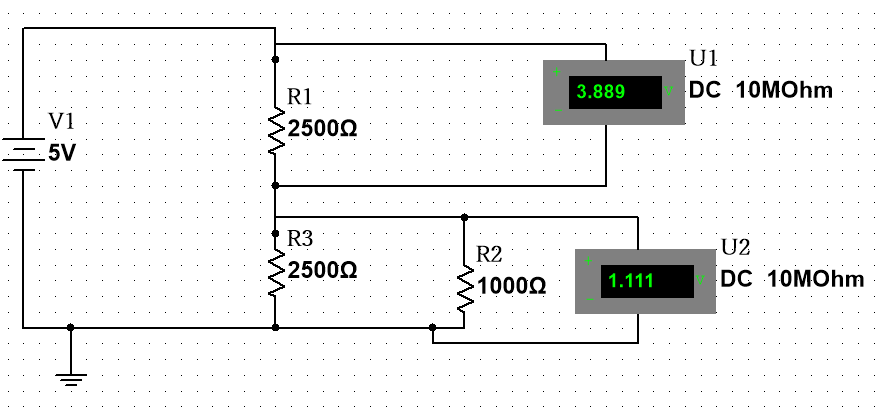
\includegraphics[width=0.4\textwidth]{images/comp.PNG}
     \caption{Comprobación del divisor de voltaje}
     \label{fig:comp}
\end{figure}

%%%%%%%%%%%%%%%%%%%%%%%%%%%EJERCICIO1%%%%%%%%%%%%%%%%%%%%%%%%%%%
\section{Ejercicios con Ley de Ohm y Leyes de Kirchhoff}
\subsection{Voltímetro y amperímetro a partir de un galvanómetro. Ejercicio1}
- Circuito mixto con divisor de corriente y divisor de voltaje. \vspace{0.5cm}\\
\noindent Tenemos los siguientes datos:
\begin{center}
    $I_{max}$ = 1A \textit{(corriente a plena escala del amperímetro)}

    $I_m$ = 1mA \textit{(corriente del galvanómetro)}

    $R_m$ = 50 $\Omega$ \textit{(resistencia máxima del galvanómetro)}
    $R_S$ = ? \textit{(resistencia interna (shunt))}

    $I_s$ = ? \textit{(corriente de derivación)}
\end{center}
\noindent Nos hace falta calcular $I_s$ y $R_s$ teniendo en cuenta las \textit{Leyes de Kirchhoff} y \textit{Ley de Ohm}.
\begin{center}
    
    I = $I_1$ + $I_2$ ... + $I_n$ \textcolor[cmyk]{1,0,1,0}{\textbf{\textit{(Ley de Kirchhoff)}}}
    
    $V_m$ = $R_m$ * $I_m$ $\Leftrightarrow$   V = $I_m$($R_s + R_m$) \textcolor[cmyk]{1,0,1,0}{\textbf{\textit{(fórmulas para calcular voltaje)}}}
    
    $R_s$ = $\frac{V}{I_s}$ \textcolor[cmyk]{1,0,1,0}{\textbf{\textit{(fórmulas para resistencia shunt)}}}

    $I_m$ = $\frac{V}{R_m}$ \textcolor[cmyk]{1,0,1,0}{\textbf{\textit{(fórmulas para resistencia del galvanómetro)}}}

    $I_s$ = $\frac{V}{R_s}$ \textcolor[cmyk]{1,0,1,0}{\textbf{\textit{(fórmula de corriente interna)}}}
\end{center}
\textit{Antes de calcular es necesario convertir las unidades para no tener errores con las operaciones.}

\begin{table}[H]
    \centering
    \begin{tabular}{|c|c|} \hline
        giga [G] & 10$^{9}$ \\ \hline
        mega [M] & 10$^{6}$ \\ \hline
        kilo [k] & 10$^{3}$ \\ \hline
        mili [m] & 10$^{-3}$ \\ \hline
        micro [$\mu$] & 10$^{-6}$ \\ \hline
        nano [n] & 10$^{-9}$ \\ \hline
    \end{tabular}
    \caption{Tabla de conversiones}\label{tabla 1}
\end{table}

\noindent Después de convertir correctamente, calculamos $I_s$ usando Ley de Kirchhoff:

\begin{center}
    $I_s = $$I_{max}$ - $I_m$
    
    $I_s$ = 1A - 0.001 A \textit{(pasando de 1mA a 1A)} 
    
    $I_s$ = 0.999 A
    
\end{center}
\noindent Calculamos el voltaje del medidor por \textit{Ley de Ohm}

\begin{center}
    V = I x R $\rightarrow$ $V_{med}$ = $I_{m}$ x $R_m$
    
    $\therefore$ V = (0.001 A) x (50 $\Omega$)
    
    V = 0.05 V (el voltaje no cambia porque es circuito paralelo)
    
\end{center}
\noindent Sacamos $R_s$ con los dos valores que sacamos antes de la misma forma usando \textit{Ley de Ohm}: 

\begin{center}
    R = $\frac{V}{I}$ $\rightarrow$ $R_s$ = $\frac{V}{I_s}$ 
    
    $\therefore$ $R_s$ = $\frac{0.05 V}{0.999 A}$
    
    R$_s$ = 0.05005 $\Omega$
    
\end{center}
\noindent Podemos hacer una comprobación usando ($R_s$)
\begin{center}
    
    V = $I_m$ ($R_s + R_m$)
    
    V = 0.001A (0.05005 $\Omega$ + 50 $\Omega$)
    
    V = 0.05 V 
\end{center}

%%%%%%%%%%%%%%%%%%%%%%%%%%%EJERCICIO2%%%%%%%%%%%%%%%%%%%%%%%%%%%

\subsection{Ejercicio2}
\noindent Tenemos los siguientes datos:
\begin{center}
    $I_{max}$ = 2A

    $I_m$ = 20$\mu$A 

    $R_m$ = 100 $\Omega$ 
\end{center}
Comenzamos calculando $I_s$:
\begin{center}
    
    $I_s$ = 2A - 0.00002 A
    
    $I_s$ = 1.99998 A
    
\end{center}
\noindent Seguimos con el voltaje: 
\begin{center}
    
    V = (0.00002 A) * (100 $\Omega$)
    
    V = 0.002 V
    
\end{center}
\noindent Sacamos la resistencia:
\begin{center}
    
    $R_s$ = $\frac{0.002 V}{1.99998 A}$
    
    $R_s$ =  0.001 $\Omega$
    
\end{center}
%%%%%%%%%%%%%%%%%%%%%%%%%%%EJERCICIO3%%%%%%%%%%%%%%%%%%%%%%%%%%%
\subsection{Ejercicio3}
\noindent Tenemos los siguientes datos:
\begin{center}
    $I_{max}$ = 10 A

    $I_m$ = 1 $\mu$A = 0.000001 A 

    $R_m$ = 100 $\Omega$ 
\end{center}

$I_s$ :
\begin{center}
    $I_s$ = 10A - 0.000001A 

    $I_s$ = 9.999999 A
\end{center}

V : 
\begin{center}
    V = (0.000001A) x (100 $\Omega$)

    V = 0.0001 $\Omega$
\end{center}

$R_s$: 
\begin{center}
    $R_s$ = $\frac{0.0001 \Omega}{9.999999}$

    $R_s$ = 0.00001 $\Omega$
\end{center}

%%%%%%%%%%%%%%%%%%%%%%%%%%%POTENCIA%%%%%%%%%%%%%%%%%%%%%%%%%%%%%
\section{Potencia}
\noindent Aquí existe mucha relación con la \textit{Ley de Ohm}:
\vspace{0.2cm}\\
I = $\frac{V}{R}$, V = IxR, R= $\frac{V}{I}$ \textcolor[cmyk]{1,0,1,0}{\textbf{\textit{(fórmulas de Ley de Ohm)}}}
\vspace{0.2cm}\\
\noindent Se sustituyen los valores en la fórmula general de potencia eléctrica: P = V x I

$\therefore$ P = V x $\frac{V}{R}$ , P = IxRxI 
\begin{center}
    Nos quedaría: P= $\frac{V^2}{R}$, P= $I^2$ x R, P= VxI \textcolor[cmyk]{1,0,1,0}{\textbf{\textit{(fórmulas de potencia)}}}
\end{center} 
\noindent En un circuito paralelo, la energía se disipa por el circuito y se desarrolla la potencia (expresada en W).

\subsection{Potencia en circuito paralelo. ejercicio1}
\noindent Tenemos una fuente de energía de 12 V y nos piden sacar la potencia de cada resistor y la potencia total.

$R_1$ = 3.6 $\Omega$ con $I_1$ = 3.333 A

$R_2$ = 220 $\Omega$ con $I_2$ = 0.055 A

$R_3$ = 100 $\Omega$ con $I_3$ = 0.12 A
\vspace{0.5cm}\\
$P_1$ = V*$I_1$= (12 V)(3.333 A)= 39.996 W

$P_2$ = V*$I_2$= (12 V)(0.055)= 0.66 W

$P_3$ = V*$I_3$= (12 V)(0.12)= 1.44 W
\vspace{0.5cm}\\
Hay dos formas para sacar la resistencia total, una de ellas es sumando todas las potencias sacadas individualmente.

\begin{center}
    $\Sigma$P = (39.996 + 0.66 + 1.44)W = 42.096 W
\end{center}
La otra forma es sacando una resistencia equivalente, es decir, en vez de usar 3 resistencias y 3 corrientes, usaremos solo una resistencia y una corriente.
\vspace{0.5cm}\\
$R_E$ = $R_1^{-1}$ + $R_2^{-1}$....$R_n^{-1}$

$R_E$ = $3.6^{-1} + 220^{-1} + 100^{-1}$

$R_E = 0.2923^{-1} \longrightarrow R_E= 3.4208 \Omega$ 
\vspace{0.5cm}\\
Para corriente equivalente se pueden sumar todas las corrientes o también:
\vspace{0.5cm}\\
$I_E = \frac{V}{R_E}$ 

$I_E = \frac{12 V}{3.4208 \Omega}$ = 3.507 W
\vspace{0.5cm}\\
Ahora fácilmente podemos calcular la potencia.

P = V*I 

P= (12 V) (3.507 A) = 42.084 W
%%%%%%%%%%%%%%%%%%%%%%%%resistenciadual%%%%%%%%%%%%%%%%%%%%%
\section{Método "dual"}
El método "dual" es reducir el circuito que tenemos gracias a la fórmula de \textit{resistencias equivalentes} que funciona exceptuando cualquier resistencia del circuito, así será más fácil obtener la \textit{corriente equivalente} cuando tenemos muchos resistores. Es lo mismo que se hizo en el ejercicio de "Circuitos mixtos", se busca la forma de simplificar/reducir el circuito para facilitar cálculos.

\noindent Recapitulando todas las fórmulas ya vistas en las secciones anteriores: 
\begin{center}

    $V_{R_n} = \frac{V*R_n}{R_T}$ \textcolor[cmyk]{1,0,1,0}{\textbf{\textit{(fórmula de divisor de voltaje)}}}
\vspace{0.3cm}\\
$R_E$ = $(R_1^{-1}$ + $R_2^{-1}$....$R_n^{-1})^{-1}$ $\leftrightsquigarrow$  $R_E = \frac{R_1R_2}{R_1+R_2}$ \textcolor[cmyk]{1,0,1,0}{\textbf{\textit{(fórmulas de resistencia equivalente o total)}}}
\vspace{0.3cm}\\
   $I_E$ = $\Sigma$ $\leftrightsquigarrow$ $I_E$ = I($\frac{R_n}{R_n+R_E}$) \textcolor[cmyk]{1,0,1,0}{\textbf{\textit{(fórmulas de corriente equivalente o total)}}}
\vspace{0.3cm}\\
I = $I_1$ + $I_2$ ... + $I_n$ \textcolor[cmyk]{1,0,1,0}{\textbf{\textit{(fórmula de Ley de Corrientes de Kirchhoff)}}}
\vspace{0.3cm}\\
I = $\frac{V}{R}$ \textcolor[cmyk]{1,0,1,0}{\textbf{\textit{(fórmula de Ley de Ohm)}}}
\vspace{0.3cm}\\
P= $\frac{V^2}{R}$, P= $I^2$ x R, P= VxI \textcolor[cmyk]{1,0,1,0}{\textbf{\textit{(fórmulas de potencia)}}}
\end{center}


%%%%%%%%%%%%%%%%%%%%%%%%%%%TODO%%%%%%%%%%%%%%%%%%%%%%%%%%%%%
\section{Ejercicios de circuitos todos los temas vistos}
\noindent A continuación tenemos el siguiente circuito paralelo:

\begin{figure}[H]
    \centering
    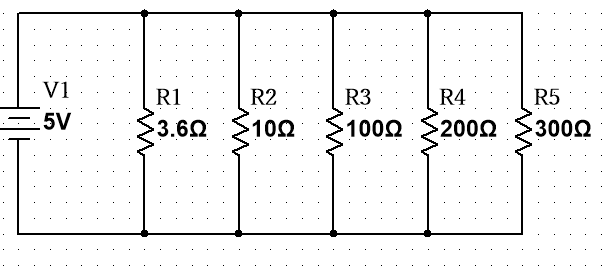
\includegraphics[width=0.5\textwidth]{images/ejercicio.PNG}
    \caption{Circuito paralelo con 5 resistores}
    \label{fg:ej}
\end{figure}
\noindent \textbf{EJERCICIO:} Calcular resistencia y corriente equivalente, potencia, corriente y potencia de cada valor de resistencia distribuida en el circuito y comprobar con el \textit{"método dual"}.
\begin{enumerate}
    \item \textbf{La resistencia equivalente o total:}
    \vspace{0.3cm}\\
    $R_E$ = ($3.6^{-1}$ + $10^{-1}$ + $100^{-1}$ +$200^{-1}$ + $300^{-1}$ )$^{-1}$$\Omega$ \textcolor[cmyk]{1,0,1,0}{\textbf{\textit{(fórmula de resistencia equivalente o total)}}}
    \vspace{0.3cm}\\
    $R_E$ = 2.52 $\Omega$
    \vspace{0.3cm}\\
    \noindent Para tener una visualización gráfica de lo que significa una "resistencia equivalente", el circuito quedaría como:

    \begin{figure}[H]
        \centering
        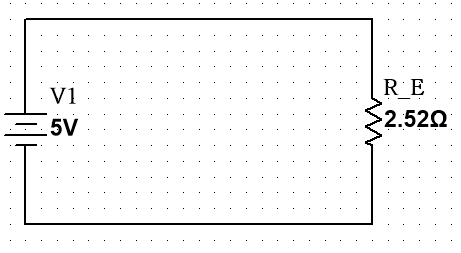
\includegraphics[width=0.4\textwidth]{images/equivalente3.PNG}
        \caption{reducción del circuito por resistencia equivalente}
        \label{fg:e1}
    \end{figure}
    \noindent De esta forma, como se explicó desde otras secciones, es mucho más fácil calcular la corriente total (o equivalente):
    \item \textbf{La corriente equivalente o total:}
    
    $I_T$ = $\frac{V}{R}$

    $I_T$ = $\frac{5V}{2.52 \Omega}$

    $I_T$ = 1.984 A 
    \item \textbf{Corriente distribuida en cada resistencia:}
    
    $I_n$ = $\frac{V}{R_n}$

    $I_1$ = $\frac{5V}{R_1}$ = $\frac{5V}{3.6 \Omega}$ = 1.38 A

    $I_2$ = $\frac{5V}{R_2}$ = $\frac{5V}{10 \Omega}$ = 0.5 A

    $I_3$ = $\frac{5V}{R_3}$ = $\frac{5V}{100 \Omega}$ = 0.05 A

    $I_4$ = $\frac{5V}{R_4}$ = $\frac{5V}{200 \Omega}$ = 0.025 A

    $I_5$ = $\frac{5V}{R_5}$ = $\frac{5V}{300 \Omega}$ = 0.016 A

    \noindent La suma de cada corriente distribuida debe ser igual a $I_T$
    \item \textbf{Potencia:}
    
    $P_T$ = V * I 

    $P_T$  = (5 V)(1.984 A) = 9.92 W
    \item \textbf{Potencia distribuida en cada valor de resistencia:}
    
    $P_n$ = $(I_n)^{2}$ * $R_n$

    $P_1$ = $(I_1)^{2}$ * $R_1$ = (1.38 A)$^{2}$ * 3.6 $\Omega$ = 6.85 W

    $P_2$ = $(I_2)^{2}$ * $R_2$ = (0.5 A)$^{2}$ * 10 $\Omega$ = 2.5 W

    $P_3$ = $(I_3)^{2}$ * $R_3$ = (0.05 A)$^{2}$ * 100 $\Omega$ = 0.25 W

    $P_4$ = $(I_4)^{2}$ * $R_4$ = (0.025 A)$^{2}$ * 200 $\Omega$ = 0.125 W

    $P_5$ = $(I_5)^{2}$ * $R_4$ = (0.016 A)$^{2}$ * 300 $\Omega$ = 0.0768 W

    \noindent La suma de todas esas potencias debe ser igual a $P_T$
    \newpage
    \item \textbf{Comprobación por el "método dual":}
    
    \noindent Reducimos el circuito dejando una resistencia de lado (no importa cual) y hacemos una resistencia equivalente con las demás.

    Vamos a empezar dejando de un lado a R1 y hacemos una resistencia equivalente de R2 a R5, visualmente sería algo así:

    \begin{figure}[H]
        \centering
        \begin{subfigure}{0.4\textwidth}
            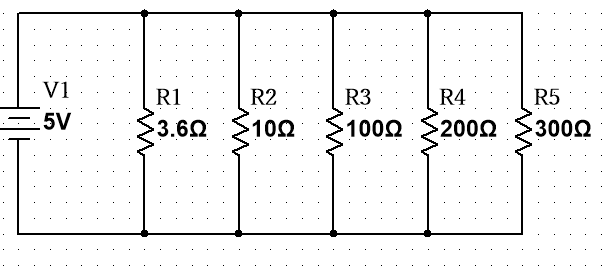
\includegraphics[width=0.9\linewidth]{images/ejercicio.PNG}
            \caption{Circuito con las 5 resistencias}
        \end{subfigure}
        \begin{subfigure}{0.3\textwidth}
            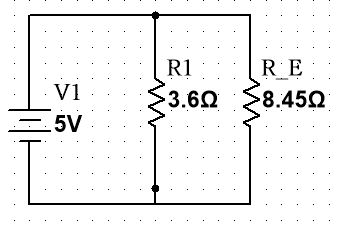
\includegraphics[width=0.9\linewidth]{images/ej.PNG}
            \caption{Circuito reducido}
        \end{subfigure}
    \end{figure}
    \noindent Matemáticamente sería:

    $R_{E1}$= $(10^{-1} + 100^{-1} + 200^{-1} + 300^{-1} )^{-1}$

    $R_{E1}$ = 8.45 $\Omega$ \textit{(resistencia equivalente)}
    \vspace{0.3cm}\\
    \noindent Para explicar mejor el "método dual", se observa que en la imagen (b) nos quedó un circuito paralelo, ya no existen 5 resistencias, ahora existen 2 y de esas 2 resistencias nos piden sacar las corrientes y potencias usando el divisor de corriente que se vió en el apartado 2.1.
    \vspace{0.3cm}\\
    Fórmula de corriente equivalente:

    $I_E$ = I($\frac{R_n}{R_n+R_E}$) es lo mismo que: $I_E$ = ($\frac{R_n*I}{R_n+R_E}$) \textit{(I=Corriente total sacada anteriormente)}
    \vspace{0.3cm}\\
    Calculamos la corriente equivalente de cada una:
    \begin{center}
        $I_{E1}$ = ($\frac{3.6 \Omega * 1.984 A}{3.6 \Omega + 8.45 \Omega}$) = 0.59 A 
    
        $I_{E2}$ = ($\frac{8.45 \Omega * 1.984 A}{3.6 \Omega + 8.45 \Omega}$) = 1.3914 A 
    \end{center}
    \noindent \textit{De forma lógica nos damos cuenta que R1 si o si debe ser menor que $R_E$ ya que en esta última se encuentran las resistencias de otras 5 más, por lo que la mayor distribución la tendra $R_E$}
    \vspace{0.3cm}\\
    \noindent La suma de esas dos corrientes debe de ser igual a la corriente total calculada anteriormente.
    \vspace{0.3cm}\\
    \noindent Se hace lo mismo para cada corriente, se deja una y sumamos las demas, eso nos dará un total de 5 circuitos paralelos los cuales debemos de sacar corriente equivalente.
\newpage
\section{Variables eléctricas}







\end{enumerate}
\end{document} %término del documento